\chapter{Triển khai bằng PyTorch và đánh giá số}
\label{chap:thucnghiem}
 
Chương~\ref{chap:pinn} đã thiết lập bằng chứng minh một loạt phát biểu về hành vi
của mạng nơ-ron thông tin vật lý: điều kiện chính quy bắt buộc lên hàm kích hoạt,
chặn ổn định nối phần dư với sai số, cơ chế khuếch đại phổ của toán tử vi phân, và
tính không khả thi của việc học trọng số cân bằng bằng hạ gradient. Mọi phát biểu
ấy đều là những khẳng định \emph{kiểm chứng được}. Chương này thực hiện việc kiểm
chứng đó.
 
Mục tiêu không dừng ở chỗ trình bày một cài đặt chạy được. Mỗi thí nghiệm dưới
đây được thiết kế để trả lời một câu hỏi cụ thể do Chương~\ref{chap:pinn} đặt ra,
với tiêu chí thành công hoặc thất bại xác định \emph{trước} khi chạy. Ta báo cáo
đầy đủ cả những chỗ khớp lẫn những chỗ không khớp: trong chín hạng mục đối chiếu
ở Mục~\ref{sec:doi-chieu}, năm khớp trọn vẹn, một khớp về hướng nhưng không về
độ lớn, một buộc phải siết lại cách phát biểu, một chỉ là tương quan chưa giải
thích được, và một cho kết quả trái với kỳ vọng.
Phần điều chỉnh được ghi rõ thay vì bỏ qua; theo quan điểm của luận văn, một kết
quả tiêu cực được phân tích đúng nguyên nhân có giá trị ngang một kết quả khớp.
 
Cấu trúc chương: Mục~\ref{sec:trienkhai} mô tả kiến trúc cài đặt trên
PyTorch~\cite{paszke2019} và cấu hình chung. Các
Mục~\ref{sec:tn1}--\ref{sec:tn6} trình bày sáu thí nghiệm.
Mục~\ref{sec:doi-chieu} đối chiếu toàn bộ lý thuyết với số liệu, và
Mục~\ref{sec:hanche} nêu thẳng những hạn chế của thiết kế thực nghiệm này.
 
%==============================================================================
\section{Kiến trúc triển khai}
\label{sec:trienkhai}
%==============================================================================
 
\subsection{Đồ thị tính toán động và vi phân tự động lồng nhau}
\label{ssec:ad-pytorch}
 
Đặc điểm khiến PyTorch phù hợp với PINNs là cơ chế \emph{đồ thị tính toán động}
(define-by-run): đồ thị theo Định nghĩa~\ref{def:comp-graph} được dựng lại ở mỗi
lượt xuôi, do đó bản thân \emph{đạo hàm} cũng là một đỉnh trong đồ thị và có thể
tiếp tục vi phân được~\cite{paszke2019}.
 
Theo Mệnh đề~\ref{md:ad-tai-tao}, việc tính $\nabla_{\btheta}r_{\btheta}$ đòi hỏi
vi phân một biểu thức vốn đã chứa $\partial_{\bxi}u_{\btheta}$. Điều kiện kỹ thuật
để thực hiện được là truyền cờ \texttt{create\_graph=True} vào
\texttt{torch.autograd.grad}: cờ này yêu cầu giữ lại đồ thị của phép tính đạo hàm
thay vì giải phóng nó. Nếu thiếu cờ, lời gọi \texttt{backward()} tiếp theo sẽ báo
lỗi hoặc -- nguy hiểm hơn -- trả về gradient bằng không mà không cảnh báo, đúng
tình huống đã nêu ở cuối Mục~\ref{subsec:bac-cao-ad}.
 
\begin{lstlisting}[caption={Toán tử đạo hàm lồng nhau theo biến đầu vào.},label={lst:grad}]
def grad(y, x, order=1):
    """Dao ham cap `order` cua y theo x, giu lai do thi de vi phan tiep."""
    for _ in range(order):
        y = torch.autograd.grad(y, x, torch.ones_like(y),
                                create_graph=True)[0]
    return y
\end{lstlisting}
 
Hàm ở Đoạn mã~\ref{lst:grad} là hiện thực trực tiếp của các công thức truy hồi
\eqref{eq:G-truy-hoi} và \eqref{eq:S-truy-hoi}: mỗi lần lặp trong vòng
\texttt{for} tương ứng với một bậc trong truy hồi Jacobi--Hessian
(Mệnh đề~\ref{md:jacobian} và \ref{md:hessian}), và chi phí nhân lên theo hệ số
hằng đúng như Nhận xét~\ref{nx:chi-phi-bac-cao} dự báo. Cần lưu ý rằng vectơ
$\texttt{torch.ones\_like(y)}$ ở đối số thứ ba chính là vectơ mầm $\bm{w}$ trong
định nghĩa biến liên hợp \eqref{eq:adjoint}: hàm này thực hiện một tích
vectơ--Jacobi \eqref{eq:vjp}, không dựng ma trận Jacobi.
 
\subsection{Mạng nơ-ron và khởi tạo}
 
\begin{lstlisting}[caption={Mạng truyền thẳng với khởi tạo Xavier và nhúng đặc trưng Fourier tuỳ chọn.},label={lst:fnn}]
class FNN(nn.Module):
    def __init__(self, layers, act="tanh", fourier_m=0, fourier_s=1.0):
        super().__init__()
        self.fourier_m = fourier_m
        if fourier_m > 0:                      # nhung dac trung Fourier
            B = torch.randn(fourier_m, layers[0]) * fourier_s
            self.register_buffer("B", B)       # B co dinh, khong hoc
            layers = [2 * fourier_m] + layers[1:]
        self.lins = nn.ModuleList(
            [nn.Linear(layers[i], layers[i+1]) for i in range(len(layers)-1)])
        for lin in self.lins:                  # khoi tao Xavier (Muc 2.3)
            nn.init.xavier_normal_(lin.weight)
            nn.init.zeros_(lin.bias)
        self.act = {"tanh": torch.tanh, "relu": torch.relu}[act]
 
    def forward(self, x):
        if self.fourier_m > 0:
            p = 2 * math.pi * x @ self.B.T
            x = torch.cat([torch.cos(p), torch.sin(p)], dim=1)
        for lin in self.lins[:-1]:
            x = self.act(lin(x))
        return self.lins[-1](x)
\end{lstlisting}
 
Ba lựa chọn trong Đoạn mã~\ref{lst:fnn} tương ứng trực tiếp với ba kết luận của
Chương~\ref{chap:fnn}. Khởi tạo Xavier là \eqref{eq:xavier} với độ chệch bằng
$\bm{0}$, đúng quy ước (A2) của Mục~\ref{subsec:phuong-sai}; ta dùng dạng
\emph{chuẩn tắc} (\texttt{xavier\_normal\_}) chứ không phải dạng đều
\eqref{eq:xavier-uniform}, và theo Nhận xét~\ref{nx:xavier-dang} hai dạng cho
cùng phương sai nên mọi kết quả của Chương~\ref{chap:fnn} áp dụng như nhau. Vòng lặp
\texttt{for lin in self.lins[:-1]} bỏ hàm kích hoạt ở lớp cuối, hiện thực quy ước
lớp ra tuyến tính \eqref{eq:fnn-output}. Ma trận $B$ của nhúng Fourier được đăng
ký bằng \texttt{register\_buffer} chứ không phải \texttt{Parameter}: nó cố định,
không tham gia tối ưu -- một quyết định thiết kế sẽ được kiểm chứng ở
Thí nghiệm~\ref{tn:pho}.
 
Toàn bộ tính toán dùng \texttt{float64}. Lựa chọn này không tuỳ tiện. Ở giai đoạn
L-BFGS, $J_r$ cần đạt tới bậc $10^{-8}$ hoặc nhỏ hơn, trong khi \texttt{float32}
chỉ có khoảng bảy chữ số thập phân có nghĩa. Quan trọng hơn, theo
Nhận xét~\ref{nx:fd-pde}, sai số ở phần dư không bị dập tắt mà được khuếch đại
qua toàn bộ quá trình huấn luyện; độ chính xác kép là điều kiện cần để phân biệt
sai số xấp xỉ với sai số làm tròn, tức để các con số trong chương này có nghĩa.
 
\subsection{Phần dư và quy trình huấn luyện hai giai đoạn}
 
\begin{lstlisting}[caption={Phần dư của phương trình Burgers và vòng huấn luyện.},label={lst:train}]
def residual(net, X):                 # X = (x, t), yeu cau requires_grad_(True)
    u  = net(X)
    g  = grad(u, X)                   # [du/dx, du/dt]
    ut, ux = g[:, 1:2], g[:, 0:1]
    uxx = grad(ux, X)[:, 0:1]         # dao ham bac hai -> can create_graph
    return ut + u * ux - NU * uxx
 
# --- Giai doan 1: Adam ---
opt = torch.optim.Adam(net.parameters(), lr=1e-3)
for it in range(adam_iters + 1):
    Jr = (residual(net, Xr) ** 2).mean()
    Jb = (net(Xb) ** 2).mean()        # hop le vi g == 0 tren bien
    J0 = ((net(X0) - u0) ** 2).mean()
    J  = Jr + lam_b * Jb + lam_0 * J0
    opt.zero_grad(); J.backward(); opt.step()
 
# --- Giai doan 2: L-BFGS voi tim kiem duong Wolfe manh ---
opt2 = torch.optim.LBFGS(net.parameters(), max_iter=800, history_size=50,
                         line_search_fn="strong_wolfe")
opt2.step(closure)
\end{lstlisting}
 
Quy trình hai giai đoạn ở Đoạn mã~\ref{lst:train} hiện thực đúng
Thuật toán~\ref{alg:two-stage}, được lập luận ở Mục~\ref{subsec:adam-vs-lbfgs}
bằng ba lý do: tính tất định của gradient, sàn nhiễu
(Mệnh đề~\ref{md:san-nhieu}), và điều kiện xấu. Tham số
\texttt{line\_search\_fn="strong\_wolfe"} không phải tuỳ chọn: theo
Bổ đề~\ref{bd:wolfe-curvature}, nó là điều kiện để $\bm{H}_k$ giữ tính xác định
dương. Hiệu quả định lượng của bước chuyển được đo ở Mục~\ref{sec:tn4}.
 
Một chi tiết cài đặt đáng nêu: dòng \texttt{Jb = (net(Xb) ** 2).mean()} chỉ đúng
vì mọi bài toán trong chương có điều kiện biên thuần nhất $g \equiv 0$. Với
$g \not\equiv 0$ phải viết \texttt{((net(Xb) - g\_b) ** 2).mean()}. Ta nêu vì đây
là lỗi im lặng: chương trình vẫn chạy và hàm mục tiêu vẫn giảm.
 
\subsection{Công cụ đo: chỉ số mất cân bằng gradient}
\label{ssec:rho}
 
Để đo bệnh lý gradient ở Mục~\ref{sec:gradient-pathology} một cách định lượng, ta
dùng chính đại lượng xuất hiện trong quy tắc \eqref{eq:lambda-hat} của
Thuật toán~\ref{alg:annealing}.
 
\begin{definition}[Chỉ số mất cân bằng gradient]
\label{dn:rho}
Với hàm mục tiêu ở dạng \eqref{eq:loss-compact}, \emph{chỉ số mất cân bằng} của
thành phần thứ $i$ tại tham số $\btheta$ là
\begin{equation}
\rho_i(\btheta)
 := \frac{\norm{\nabla_{\btheta} J_r(\btheta)}_{\infty}}
         {\tfrac{1}{P}\norm{\nabla_{\btheta} J_i(\btheta)}_{1}} .
\label{eq:rho}
\end{equation}
Ta nói bài toán \emph{mắc bệnh lý gradient} đối với thành phần $i$ nếu
$\rho_i \gg 1$ \emph{và} $\rho_i$ tăng theo số vòng lặp huấn luyện.
\end{definition}
 
Điều kiện thứ hai trong Định nghĩa~\ref{dn:rho} là điều kiện thực chất và cần
được nhấn mạnh, vì bài toán khuếch tán ở Mục~\ref{sec:tn4} sẽ cho thấy một
bài toán có
$\rho_b = 25{,}4$ tại khởi tạo nhưng \emph{giảm} sau đó, và việc can thiệp vào bài
toán ấy phản tác dụng. Giá trị tuyệt đối của $\rho_i$ tại một thời điểm không đủ
để chẩn đoán; xu hướng mới đủ.
 
\begin{lstlisting}[caption={Đo chỉ số mất cân bằng $\rho_i$ theo \eqref{eq:rho}.},label={lst:rho}]
def imbalance(loss_r, loss_i, params):
    """rho_i = max|grad J_r| / mean|grad J_i|   (Dinh nghia 5.1)."""
    gr = flat_grad(loss_r, params)     # can retain_graph=True
    gi = flat_grad(loss_i, params)
    return gr.abs().max().item() / gi.abs().mean().item()
\end{lstlisting}
 
Theo Mệnh đề~\ref{md:chi-phi-bp}, mỗi lượt ngược riêng rẽ tốn xấp xỉ chi phí một
lượt xuôi, nên việc đo $\rho_i$ đắt gấp $M+1$ lần một bước huấn luyện thường. Ta
chỉ đo mỗi $100$ vòng lặp.
 
\subsection{Cấu hình thí nghiệm và chỉ tiêu đánh giá}
\label{ssec:cauhinh}
 
\begin{table}[H]
\centering
\caption{Cấu hình chung của các thí nghiệm. Mọi lần chạy dùng hạt giống cố định
để tái lập được; hạn chế của lựa chọn này được nêu ở Mục~\ref{sec:hanche}.}
\label{tab:cauhinh}
\small
\begin{tabular}{@{}p{4.3cm}p{9.2cm}@{}}
\toprule
\textbf{Hạng mục} & \textbf{Thiết lập} \\
\midrule
Thư viện & PyTorch, NumPy; độ chính xác \texttt{float64} \\
Phần cứng & 1 lõi CPU, không dùng GPU \\
Hàm kích hoạt & $\tanh$ (trừ thí nghiệm đối chứng ReLU ở Mục~\ref{sec:tn1}) \\
Khởi tạo & Xavier dạng chuẩn tắc, $\Var(w^{(\ell)}) = 2/(n_{\ell-1}+n_{\ell})$
  theo \eqref{eq:xavier}; $\bb^{(\ell)} = \bm{0}$ \\
Kiến trúc bài toán 1D & $(1,32,32,32,1)$, $2\,209$ tham số \\
Kiến trúc bài toán 2D & $(2,32,32,32,32,1)$, $3\,297$ tham số \\
Kiến trúc bài toán đa tần số & $(1,64,64,64,1)$, $8\,513$ tham số \\
Tối ưu giai đoạn 1 & Adam, $\eta = 10^{-3}$, $\beta = (0{,}9;\,0{,}999)$ \\
Tối ưu giai đoạn 2 & L-BFGS, \texttt{history\_size}${}=50$, Wolfe mạnh \\
Lấy mẫu điểm phối trí & Lưới đều (1D) hoặc lấy mẫu đều ngẫu nhiên (2D) \\
\bottomrule
\end{tabular}
\end{table}
 
Số tham số trong Bảng~\ref{tab:cauhinh} khớp với công thức \eqref{eq:so-tham-so}:
với kiến trúc $(1,32,32,32,1)$ ta có
$P = (1\cdot32+32) + 2\times(32\cdot32+32) + (32\cdot1+1) = 64 + 2112 + 33
= 2\,209$.
 
\begin{definition}[Chỉ tiêu sai số]
\label{dn:chi-tieu}
Gọi $\{\bxi_j\}_{j=1}^{M}$ là lưới đánh giá, \emph{khác} với tập điểm phối trí
huấn luyện, và $u^{\star}$ là nghiệm đúng hoặc nghiệm tham chiếu. Ta dùng
\begin{equation}
\varepsilon_{L^2}
 := \frac{\Big(\sum_{j}\abs{u_{\btheta}(\bxi_j)
      - u^{\star}(\bxi_j)}^2\Big)^{1/2}}
         {\Big(\sum_{j}\abs{u^{\star}(\bxi_j)}^2\Big)^{1/2}},
\qquad
\varepsilon_{L^{\infty}}
 := \max_{j}\abs{u_{\btheta}(\bxi_j) - u^{\star}(\bxi_j)}.
\label{eq:chi-tieu}
\end{equation}
\end{definition}
 
Việc đánh giá trên lưới \emph{khác} tập huấn luyện là bắt buộc chứ không phải cẩn
trọng thừa. Nhận xét~\ref{rem:monte-carlo} đã lập luận rằng $J_r$ mất tính không
chệch ngay khi $\btheta$ được tối ưu trên chính tập mẫu sinh ra nó: giá trị $J_r$
cuối cùng là ước lượng chệch xuống của $\norm{r_{\btheta}}^2_{L^2}$. Sai số đo
trên lưới độc lập mới phản ánh chất lượng nội suy thực sự.
 
%==============================================================================
\section{Thí nghiệm 1: hàm kích hoạt và sự suy biến của ReLU}
\label{sec:tn1}
%==============================================================================
 
\begin{thinghiem}[Kiểm chứng Hệ quả~\ref{hq:pinn-hong}]
\label{tn:relu}
Hệ quả~\ref{hq:pinn-hong} khẳng định mạng ReLU cho
$\partial_{xx}u_{\btheta} = 0$ hầu khắp nơi
(Hệ quả~\ref{hq:relu-hkn}), dẫn tới $J_r$ hằng địa phương với giá trị
$\overline{f^2}$ và $\nabla_{\btheta}J_r \equiv \bm{0}$. Đây là khẳng định về
\emph{đẳng thức chính xác}, không phải về ``hội tụ chậm'', nên có thể kiểm chứng
tới từng chữ số máy.
\end{thinghiem}
 
\textbf{Thiết lập.} Bài toán Poisson một chiều với nghiệm chế tạo:
\begin{equation}
-u''(x) = f(x) \ \text{ trên } (0,1),
\qquad u(0) = u(1) = 0,
\qquad u^{\star}(x) = \sin(2\pi x),
\label{eq:poisson-tn1}
\end{equation}
do đó $f(x) = 4\pi^2\sin(2\pi x)$. Đây chính là bài toán của
Mệnh đề~\ref{md:chan-on-dinh}, nên ta có sẵn chặn ổn định
$\norm{e_{\btheta}}_{L^2} \le \pi^{-2}\norm{r_{\btheta}}_{L^2}$ để đối chiếu.
Huấn luyện $4\,000$ vòng Adam với $256$ điểm phối trí đều, $\lambda_b = 100$, hai
hàm kích hoạt $\tanh$ và ReLU trên cùng kiến trúc và cùng hạt giống.
 
\begin{table}[H]
\centering
\caption{So sánh hai hàm kích hoạt trên bài toán Poisson \eqref{eq:poisson-tn1}.}
\label{tab:tn1}
\small
\begin{tabular}{@{}lrrrr@{}}
\toprule
\textbf{Hàm kích hoạt} & $\varepsilon_{L^2}$ & $\varepsilon_{L^{\infty}}$
& $J_r$ cuối & $\norm{\nabla_{\btheta}J_r}_{\infty}$ \\
\midrule
$\tanh$ & $5{,}977\times10^{-5}$ & $8{,}701\times10^{-5}$
        & $2{,}463\times10^{-3}$ & --- \\
ReLU    & $9{,}991\times10^{-1}$ & $1{,}004\times10^{0}$
        & $7{,}762\times10^{2}$  & $0{,}0$ \\
\bottomrule
\end{tabular}
\end{table}
 
\textbf{Kết quả.} Ba con số dưới đây là bằng chứng trực tiếp cho từng khẳng định
của Hệ quả~\ref{hq:pinn-hong}.
 
\begin{enumerate}[label=(\alph*),leftmargin=2.2em,itemsep=3pt]
\item \emph{Đạo hàm bậc hai triệt tiêu.} Đo trực tiếp trên mạng ReLU tại khởi tạo
cho $\max_{x}\abs{\partial_{xx}u_{\btheta}(x)} = 0{,}0$ \emph{chính xác} -- không
phải một số nhỏ -- vì \texttt{autograd} truyền $\sigma'' \equiv 0$ qua toàn bộ đồ
thị, đúng theo truy hồi \eqref{eq:ad-hvp}: số hạng thứ nhất triệt tiêu ở mọi lớp,
số hạng thứ hai không có gì để truyền.
 
\item \emph{Hàm mục tiêu hằng.} Giá trị đo được $J_r = 776{,}229$. Đối chiếu:
giá trị liên tục là
$\overline{f^2} = \int_0^1 16\pi^4\sin^2(2\pi x)\,dx = 8\pi^4 = 779{,}273$, còn
trung bình của $f^2$ \emph{trên đúng lưới đánh giá $1\,001$ điểm} là
$778{,}494$. Sai lệch giữa $776{,}229$ và $778{,}494$ là $0{,}29\%$, do hai lưới
cầu phương khác nhau ($256$ điểm huấn luyện so với $1\,001$ điểm đánh giá) chứ
không do mạng. Ta nêu cả hai giá trị tham chiếu vì việc chỉ nêu một trong hai dễ
gây hiểu nhầm về nguồn sai lệch.
 
\item \emph{Gradient triệt tiêu.} $\norm{\nabla_{\btheta}J_r}_{\infty} = 0{,}0$
và $\norm{\nabla_{\btheta}J_r}_{2} = 0{,}0$, đúng bằng không trong số học dấu
phẩy động -- không phải nhỏ dưới một ngưỡng.
\end{enumerate}
 
Sai số $\varepsilon_{L^2} = 0{,}9991 \approx 1$ của mạng ReLU có nghĩa hình học
rõ ràng: mạng hội tụ về $u_{\btheta} \approx 0$. Nó chỉ học được điều kiện biên --
thành phần duy nhất còn gradient -- và hoàn toàn mù trước phương trình. Chênh lệch
độ chính xác giữa hai hàm kích hoạt là $1{,}67\times 10^{4}$ lần.
 
\begin{figure}[H]
\centering
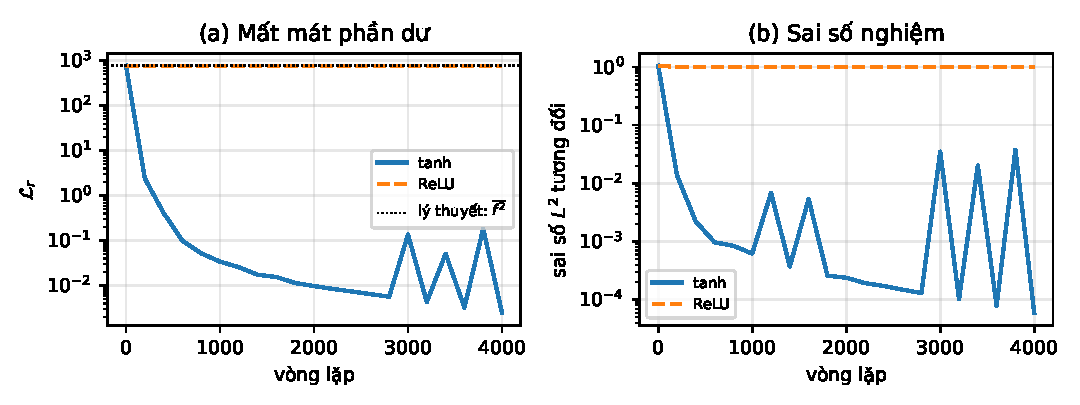
\includegraphics[width=\textwidth]{Images/chap_5/fig51_relu.pdf}
\caption{Bài toán Poisson \eqref{eq:poisson-tn1} với hai hàm kích hoạt. (a) Mất
mát phần dư của mạng ReLU nằm đúng trên đường lý thuyết $\overline{f^2}$ và không
hề giảm suốt $4\,000$ vòng lặp. (b) Sai số $L^2$ tương ứng.}
\label{fig:tn1}
\end{figure}
 
\begin{nhanxet}[Dấu hiệu chẩn đoán]
Hình~\ref{fig:tn1}(a) cho một quy tắc thực dụng: nếu $J_r$ của một PINN nằm phẳng
tuyệt đối \emph{ngay từ vòng lặp đầu tiên}, nguyên nhân gần như chắc chắn là bậc
khả vi của hàm kích hoạt thấp hơn bậc của toán tử vi phân, chứ không phải tốc độ
học hay khởi tạo. Dấu hiệu phân biệt là chữ ``ngay từ đầu'': một bài toán khó
nhưng đúng kiến trúc vẫn giảm $J_r$ ở những vòng đầu rồi mới chững lại theo cơ chế
sàn nhiễu (Mệnh đề~\ref{md:san-nhieu}).
\end{nhanxet}
 
%==============================================================================
\section{Thí nghiệm 2: cái giá của ràng buộc mềm}
\label{sec:tn2}
%==============================================================================
 
Nhận xét~\ref{rem:soft-constraint} đã nêu rằng ràng buộc mềm không được thoả
chính xác, nhưng chưa lượng hoá mức vi phạm. Mệnh đề sau lấp chỗ trống đó; nó là
dạng chuyên biệt hoá của kết quả cổ điển về phương pháp phạt toàn
phương~\cite{nocedal2006}.
 
\begin{menhde}[Sai số biên của phương pháp phạt]
\label{md:phat-bien-phat}
Xét $J_{\lambda}(\btheta) = J_r(\btheta) + \lambda\, c(\btheta)^2$ với
$J_r, c \in C^1$, và giả sử $\btheta_{\lambda}$ là một điểm dừng của
$J_{\lambda}$. Nếu tồn tại các hằng số $0 < a \le A$ và $G$ sao cho
$a \le \norm{\nabla c(\btheta_{\lambda})} \le A$ và
$\norm{\nabla J_r(\btheta_{\lambda})} \le G$ với mọi $\lambda$ đủ lớn, thì
\begin{equation}
\abs{c(\btheta_{\lambda})} \;\le\; \frac{G}{2a}\cdot\frac{1}{\lambda}
 \;=\; \mathcal{O}\!\left(\lambda^{-1}\right).
\label{eq:phat-bac-nhat}
\end{equation}
\end{menhde}
 
\begin{proof}
Điều kiện dừng $\nabla J_{\lambda}(\btheta_{\lambda}) = \bm{0}$ cho
\[
\nabla J_r(\btheta_{\lambda})
 + 2\lambda\, c(\btheta_{\lambda})\,\nabla c(\btheta_{\lambda}) = \bm{0}
\quad\Longrightarrow\quad
2\lambda\,\abs{c(\btheta_{\lambda})}\,\norm{\nabla c(\btheta_{\lambda})}
 = \norm{\nabla J_r(\btheta_{\lambda})} .
\]
Thay chặn dưới $\norm{\nabla c} \ge a$ và chặn trên
$\norm{\nabla J_r} \le G$, rồi chia hai vế cho $2\lambda a$.
\end{proof}
 
Hai giả thiết của Mệnh đề~\ref{md:phat-bien-phat} đáng chú ý. Giả thiết
$\norm{\nabla c} \ge a > 0$ là điều kiện chính quy của ràng buộc; nếu nó hỏng,
quan hệ $\lambda^{-1}$ hỏng theo. Giả thiết $\norm{\nabla J_r} \le G$ nói rằng
gradient phần dư không bùng nổ khi $\lambda$ tăng -- một giả thiết mà chính thí
nghiệm dưới đây sẽ cho thấy bị vi phạm ở đầu $\lambda_b$ lớn.
 
\begin{thinghiem}[Kiểm chứng Mệnh đề~\ref{md:phat-bien-phat}]
\label{tn:lambda}
Quy luật $\lambda_b^{-1}$ được chứng minh cho một điểm dừng chính xác của một mô
hình một ràng buộc. Câu hỏi: nó có sống sót trên bài toán phi tuyến thật, với
$2\,209$ tham số và tối ưu chưa hội tụ hoàn toàn hay không?
\end{thinghiem}
 
\textbf{Thiết lập.} Vẫn bài toán \eqref{eq:poisson-tn1}, cố định
$\lambda_r = 1$ và quét $\lambda_b$ qua sáu bậc độ lớn. Đại lượng đo là
$\max\{\abs{u_{\btheta}(0)}, \abs{u_{\btheta}(1)}\}$.
 
\begin{table}[H]
\centering
\caption{Ảnh hưởng của trọng số biên $\lambda_b$ (bài toán Poisson, $4\,000$ vòng
Adam). Giá trị tốt nhất của mỗi cột được in đậm.}
\label{tab:tn2}
\small
\begin{tabular}{@{}rrrrr@{}}
\toprule
$\lambda_b$ & sai số biên & $\varepsilon_{L^2}$ & $\varepsilon_{L^{\infty}}$
& $J_r$ \\
\midrule
$0{,}01$ & $9{,}117\times10^{-1}$ & $7{,}455\times10^{-1}$
         & $9{,}117\times10^{-1}$ & $2{,}933\times10^{-3}$ \\
$0{,}1$  & $1{,}743\times10^{-2}$ & $1{,}422\times10^{-2}$
         & $1{,}743\times10^{-2}$ & $2{,}415\times10^{-3}$ \\
$1$      & $8{,}033\times10^{-4}$ & $5{,}488\times10^{-4}$
         & $8{,}033\times10^{-4}$ & $2{,}171\times10^{-4}$ \\
$10$     & $1{,}858\times10^{-4}$ & $1{,}437\times10^{-4}$
         & $2{,}053\times10^{-4}$ & $9{,}301\times10^{-4}$ \\
$100$    & $2{,}697\times10^{-5}$ & $\mathbf{5{,}977\times10^{-5}}$
         & $8{,}701\times10^{-5}$ & $2{,}463\times10^{-3}$ \\
$1\,000$ & $\mathbf{1{,}180\times10^{-5}}$ & $3{,}300\times10^{-4}$
         & $3{,}313\times10^{-4}$ & $1{,}028\times10^{-2}$ \\
\bottomrule
\end{tabular}
\end{table}
 
\textbf{Kết quả.} Hồi quy tuyến tính trên thang log--log trong dải
$\lambda_b \in [0{,}1;\,100]$ cho
\begin{equation}
\text{sai số biên} \;\propto\; \lambda_b^{-0{,}907},
\label{eq:do-doc-do}
\end{equation}
so với số mũ $-1$ của Mệnh đề~\ref{md:phat-bien-phat}. Sai lệch $9\%$ ở số mũ là
mức phù hợp tốt, xét rằng mệnh đề được chứng minh tại một \emph{điểm dừng chính
xác} của mô hình một ràng buộc, còn thực nghiệm chạy trên mạng phi tuyến
$2\,209$ tham số sau $4\,000$ vòng Adam -- tức tại một điểm mà theo
Mệnh đề~\ref{md:san-nhieu}, gradient chưa triệt tiêu mà chỉ dao động quanh sàn
nhiễu.
 
Ở đầu $\lambda_b = 0{,}01$, sai số biên bão hoà ở mức $0{,}91$: đúng kịch bản
Nhận xét~\ref{rem:ill-posedness} mô tả. Nghiệm thu được thoả phương trình khá tốt
-- $J_r$ thậm chí nhỏ nhất trong bảng -- nhưng sai hoàn toàn ở biên, tức mạng đã
trôi trên tập $\mathcal{M}_r$ của \eqref{eq:manifold-r} và hội tụ về \emph{một
nghiệm khác} của cùng phương trình vi phân. Đây cũng là minh hoạ cụ thể cho việc
vì sao Mệnh đề~\ref{md:chan-on-dinh} phải giả thiết điều kiện biên thoả chính
xác: ở dòng này, phần dư nhỏ mà sai số lớn.
 
\begin{figure}[H]
\centering
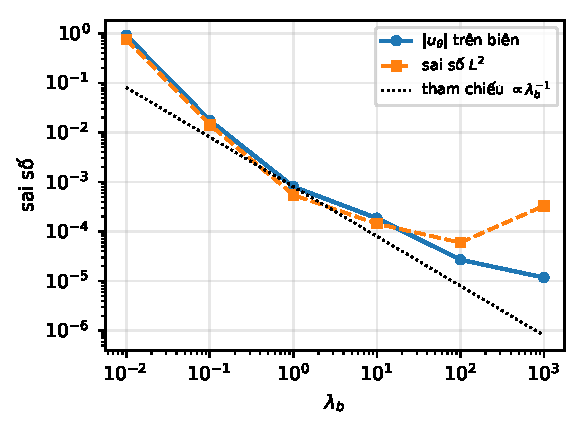
\includegraphics[width=0.55\textwidth]{Images/chap_5/fig52_lambda.pdf}
\caption{Sai số biên và sai số $L^2$ theo $\lambda_b$. Đường chấm là tham chiếu
$\propto \lambda_b^{-1}$ của Mệnh đề~\ref{md:phat-bien-phat}.}
\label{fig:tn2}
\end{figure}
 
\begin{nhanxet}[Đánh đổi mà Mệnh đề~\ref{md:phat-bien-phat} không nắm bắt]
\label{nx:danh-doi}
Cột $\varepsilon_{L^2}$ của Bảng~\ref{tab:tn2} bộc lộ một hiện tượng nằm ngoài
phạm vi mệnh đề. Khi $\lambda_b$ tăng từ $100$ lên $1\,000$, sai số biên tiếp tục
giảm ($2{,}70\times10^{-5} \to 1{,}18\times10^{-5}$) đúng như dự báo, nhưng sai số
$L^2$ \emph{toàn cục lại xấu đi} $5{,}5$ lần
($5{,}98\times10^{-5} \to 3{,}30\times10^{-4}$), đồng thời $J_r$ tăng $4{,}2$
lần.
 
Lý do là Mệnh đề~\ref{md:phat-bien-phat} chỉ theo dõi \emph{một} trong hai mục
tiêu cạnh tranh, và giả thiết $\norm{\nabla J_r} \le G$ của nó bị vi phạm: cột
$J_r$ cho thấy phần dư tăng đơn điệu từ $\lambda_b = 1$ trở đi. Khi $\lambda_b$
quá lớn, điểm tối ưu bị đẩy về đầu kia của đường đánh đổi: điều kiện biên gần như
chính xác, nhưng phần dư trong miền bị hy sinh.
 
Kết luận thực hành: $\lambda_b$ tối ưu theo nghĩa sai số toàn cục là một giá trị
\emph{hữu hạn} -- ở đây $\lambda_b \approx 100$ -- chứ không phải càng lớn càng
tốt. Đây là bổ sung của thực nghiệm cho phân tích lý thuyết ở
Mục~\ref{sec:gradient-pathology}, và nó sẽ tái xuất ở
Mục~\ref{sec:tn4}--\ref{sec:tn5} dưới dạng nguyên nhân khiến thuật toán ủ trọng
số phản tác dụng.
\end{nhanxet}
 
%==============================================================================
\section{Thí nghiệm 3: thiên kiến phổ và sự đảo chiều do toán tử vi phân}
\label{sec:tn3}
%==============================================================================
 
Đây là thí nghiệm quan trọng nhất của chương, vì nó buộc phải siết lại một kết
luận của Chương~\ref{chap:pinn}.
 
\paragraph{Giả thuyết làm việc.}
Chương~\ref{chap:pinn} cho hai thừa số tác động lên tốc độ học của một mode tần
số $\bk$, nhưng chưa ghép chúng thành một công thức. Một mặt,
Nhận xét~\ref{rem:ntk-view} cho tốc độ phân rã của mode thứ $j$ trong bài toán
hồi quy là trị riêng $\varkappa_j$ của nhân tiếp tuyến; viết
$\widehat{\varkappa}(\bk)$ cho ký hiệu phổ của nhân. Mặt khác,
Mệnh đề~\ref{md:khuech-dai} cho biết hàm mục tiêu phần dư nhìn thấy sai số qua ký
hiệu chính $P(\bk)$ của toán tử, với biên độ bị nhân lên $\abs{P(\bk)}$. Vì hàm mục tiêu là bình phương, ta \emph{giả thuyết} rằng tốc độ hiệu dụng là
\begin{equation}
\mu(\bk) \;=\; \abs{P(\bk)}^{2}\,\widehat{\varkappa}(\bk).
\label{eq:pho-hieu-dung}
\end{equation}
Cần nói thẳng: \eqref{eq:pho-hieu-dung} \emph{không} phải một mệnh đề đã chứng
minh trong luận văn. Nó là giả thuyết làm việc ghép từ hai kết quả nói trên, và
mục đích của thí nghiệm này là kiểm tra dự báo định tính của nó.
 
Dự báo ấy như sau. Với toán tử Poisson trong $\R^1$, $P(k) = 4\pi^2k^2$, nên
$\abs{P(k)}^{2} \propto k^{4}$. Nếu $\widehat{\varkappa}(k)$ suy giảm chậm hơn
$k^{-4}$ thì $\mu(k)$ \emph{tăng} theo $k$: hàm mục tiêu phần dư sẽ \emph{ưu tiên
tần số cao} -- ngược hẳn với thiên kiến phổ cổ điển của
Định lý~\ref{dl:spectral-decay}.
 
\begin{thinghiem}[Kiểm tra giả thuyết \eqref{eq:pho-hieu-dung}]
\label{tn:pho}
Đo thứ tự học các mode tần số trên cùng một nghiệm đích, dưới hai hàm mục tiêu
khác nhau: hồi quy ($P \equiv 1$) và phần dư ($P(k) = 4\pi^2k^2$). Nếu
\eqref{eq:pho-hieu-dung} đúng về hướng, hai chế độ phải cho thứ tự học
\emph{ngược nhau}.
\end{thinghiem}
 
\textbf{Thiết lập.} Nghiệm chế tạo đa tần số với biên độ bằng nhau trên $(0,1)$:
\begin{equation}
u^{\star}(x) = \sum_{k \in \{1,4,8\}} \sin(2\pi k x),
\qquad
f(x) = \sum_{k \in \{1,4,8\}} 4\pi^2 k^2 \sin(2\pi k x).
\label{eq:da-tan-so}
\end{equation}
Biên độ bằng nhau là điều kiện thiết kế then chốt: nó bảo đảm mọi khác biệt về
thứ tự học đến từ hàm mục tiêu chứ không từ trọng số ban đầu của các mode. Ba chế
độ huấn luyện trên \emph{cùng} mục tiêu, cùng kiến trúc, cùng hạt giống:
 
\begin{enumerate}[label=(\alph*),leftmargin=2.2em,itemsep=2pt]
\item \textbf{Hồi quy}: $J = \overline{\abs{u_{\btheta} - u^{\star}}^2}$, tức
$P \equiv 1$ và $\mu(k) = \widehat{\varkappa}(k)$. Đây là nhóm đối chứng, đo
thiên kiến phổ \emph{thuần tuý của mạng}.
\item \textbf{Phần dư}: $J = \overline{\abs{-u_{\btheta}'' - f}^2} + 100\,J_b$,
tức $\mu(k) = \abs{P(k)}^2\widehat{\varkappa}(k)$ theo
\eqref{eq:pho-hieu-dung}.
\item \textbf{Phần dư kèm đặc trưng Fourier}: như (b) nhưng thêm nhúng của
Bảng~\ref{tab:remedies} với $M = 32$, $s = 6$.
\end{enumerate}
 
Đại lượng theo dõi là hệ số sai số theo từng mode,
\begin{equation}
c_k(n) = 2\int_0^1 \big(u_{\btheta_n} - u^{\star}\big)\sin(2\pi k x)\,dx,
\label{eq:he-so-mode}
\end{equation}
hợp lệ vì $\int_0^1\sin^2(2\pi kx)\,dx = \tfrac12$, cùng
$t_{10}(k) :=$ số vòng lặp đầu tiên để $\abs{c_k}$ giảm còn $10\%$ giá trị ban
đầu.
 
\begin{table}[H]
\centering
\caption[Thứ tự học các mode tần số]{Thứ tự học các mode tần số. Dấu ``---''
nghĩa là không đạt ngưỡng trong $8\,000$ vòng lặp. \textbf{Cảnh báo khi đọc:}
$t_{10}$ là thời điểm $\abs{c_k}$ chạm ngưỡng $10\%$ \emph{lần đầu}, và đại
lượng này \emph{không đơn điệu} -- một mode có thể đạt ngưỡng rồi bị đẩy ra xa
trở lại. Ở chế độ (b), mode $k=1$ chạm ngưỡng tại vòng $200$ nhưng sau đó phân
kỳ tới $\abs{c_1} = 6{,}605$ tại vòng $40\,000$ theo \eqref{eq:c-plateau}. Vì
vậy cột $t_{10}$ \emph{không} phản ánh thứ tự học của chế độ (b); căn cứ đúng là
\eqref{eq:c-plateau}.}
\label{tab:tn3}
\small
\begin{tabular}{@{}lrrrr@{}}
\toprule
\textbf{Chế độ} & $t_{10}(k{=}1)$ & $t_{10}(k{=}4)$ & $t_{10}(k{=}8)$
& $\varepsilon_{L^2}$ \\
\midrule
(a) Hồi quy trực tiếp   & $700$    & $1\,100$ & $2\,100$
                        & $7{,}105\times10^{-3}$ \\
(b) Mất mát phần dư     & $200$    & ---      & ---
                        & $5{,}465\times10^{0}$ \\
(c) Phần dư + Fourier   & $4\,200$ & $100$    & $100$
                        & $3{,}393\times10^{-2}$ \\
\bottomrule
\end{tabular}
\end{table}
 
\begin{figure}[H]
\centering
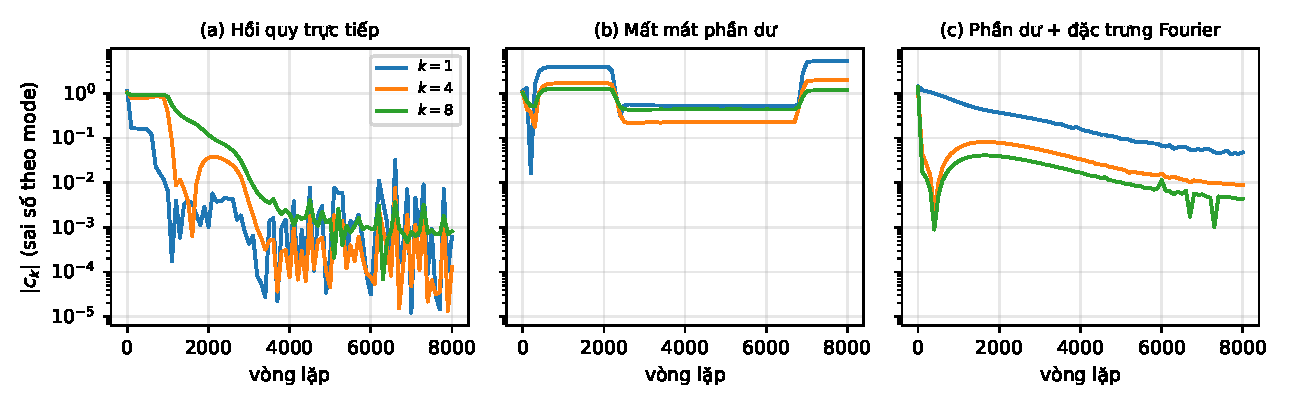
\includegraphics[width=\textwidth]{Images/chap_5/fig53_spectral.pdf}
\caption{Sai số theo từng mode tần số $\abs{c_k}$ trong ba chế độ huấn luyện trên
cùng nghiệm đích \eqref{eq:da-tan-so}.}
\label{fig:tn3}
\end{figure}
 
\textbf{Kết quả và phân tích.}
 
\emph{(a) Thiên kiến phổ cổ điển được xác nhận.} Chế độ hồi quy cho thứ tự học
đơn điệu theo tần số: $700 < 1\,100 < 2\,100$ vòng lặp cho $k = 1, 4, 8$, với tỉ
lệ $t_{10}(8)/t_{10}(1) = 3{,}0$. Đây đúng là nội dung của
Nhận xét~\ref{rem:ntk-view} với $\widehat{\varkappa}$ suy giảm theo tần số, và là
biểu hiện động lực học của Hệ quả~\ref{hq:parameter-cost}.
 
\emph{(b) Toán tử vi phân đảo ngược thứ tự ưu tiên.} Chế độ phần dư thất bại:
$\varepsilon_{L^2} = 5{,}465$, tức sai số lớn hơn cả biên độ nghiệm. Điều đáng nói
là \emph{cấu trúc} của sai số. Một lần chạy đối chứng kéo dài tới $40\,000$ vòng
cho thấy quá trình dừng hẳn từ vòng $20\,000$ (giá trị $\varepsilon_{L^2}$ tại các
mốc $20\,000$, $30\,000$, $40\,000$ lần lượt là $5{,}474$, $5{,}475$, $5{,}475$),
và phân tích theo mode tại vòng $40\,000$ cho
\begin{equation}
\abs{c_1} = 6{,}605,
\qquad
\abs{c_4} = 0{,}821,
\qquad
\abs{c_8} = 0{,}171 .
\label{eq:c-plateau}
\end{equation}
Trong ba mode được theo dõi, sai số tập trung ở mode \emph{tần số thấp nhất}, còn
mode tần số cao nhất được học tốt nhất, với tỉ lệ
$\abs{c_1}/\abs{c_8} = 38{,}6$. Đây đúng là hướng mà \eqref{eq:pho-hieu-dung} dự
báo.

Kết luận này \emph{mâu thuẫn bề ngoài} với cột $t_{10}$ của
Bảng~\ref{tab:tn3}, nơi chế độ (b) cho $t_{10}(k{=}1) = 200$ -- nhanh nhất trong
ba mode -- còn $k = 4$ và $k = 8$ không đạt ngưỡng. Cần giải thích rõ chỗ này vì
nó dễ dẫn tới kết luận ngược. Hai cột đo hai thứ khác nhau: $t_{10}$ là thời
điểm \emph{chạm ngưỡng lần đầu}, còn \eqref{eq:c-plateau} là sai số \emph{tại
điểm dừng}. Với hàm mục tiêu phần dư, quỹ đạo của $\abs{c_1}$ không đơn điệu --
nó giảm qua ngưỡng $10\%$ ở vòng $200$ rồi \emph{bị đẩy ngược trở ra} và ổn định
ở $6{,}605$, tức lớn gấp hơn sáu lần biên độ ban đầu của chính mode đó. Trong
khi ấy $\abs{c_4} = 0{,}821$ và $\abs{c_8} = 0{,}171$ tuy chưa bao giờ chạm
ngưỡng $10\%$ nhưng dừng ở mức thấp hơn hẳn. Vì mục tiêu của thí nghiệm là so
sánh thứ tự \emph{ưu tiên} chứ không phải tốc độ chạm một ngưỡng tuỳ chọn, căn
cứ đúng là \eqref{eq:c-plateau}; cột $t_{10}$ chỉ đọc được như một chỉ báo thứ
tự ở chế độ (a) và (c), nơi nó nhất quán với sai số cuối cùng.
 
Về độ lớn, cần tách hai con số thường bị lẫn. Thừa số $\abs{P(k)}^2 \propto k^4$
\emph{một mình} ưu tiên mode $k=8$ hơn mode $k=1$ một hệ số $8^4 = 4\,096$. Nhưng
$\mu(k)$ trong \eqref{eq:pho-hieu-dung} còn chứa $\widehat{\varkappa}(k)$, vốn suy
giảm theo $k$; với ước lượng thô $\widehat{\varkappa}(k)\sim k^{-2}$ ta được
$\mu(k) \sim k^{2}$ và hệ số ưu tiên chỉ còn $8^2 = 64$. Tỉ lệ đo được $38{,}6$
nằm gần con số thứ hai hơn -- nhưng ta không rút kết luận định lượng từ đối chiếu
này, vì $\abs{c_k}$ tại điểm dừng không phải một hàm đơn giản của $\mu(k)$, và vì
ước lượng $\widehat{\varkappa}(k)\sim k^{-2}$ chưa được chứng minh ở đâu trong
luận văn.
 
\begin{nhanxet}[Ba mode được theo dõi không chiếm hết sai số]
\label{nx:nang-luong}
Một đối chiếu nhất quán nội tại đáng làm. Vì
$\norm{u^{\star}}^2_{L^2(0,1)} = 3/2$, sai số tương đối $5{,}465$ tương ứng
$\norm{e_{\btheta}}^2_{L^2} = 5{,}465^2\times 1{,}5 = 44{,}80$. Trong khi đó ba
mode ở \eqref{eq:c-plateau} chỉ đóng góp
$\tfrac12(6{,}605^2 + 0{,}821^2 + 0{,}171^2) = 22{,}16$, tức $49{,}5\%$ tổng năng
lượng sai số.
 
Vậy khoảng một nửa sai số nằm ở các thành phần \emph{ngoài} ba mode được theo dõi
-- nhiều khả năng là thành phần hằng và các mode tần số thấp khác, những thành
phần mà toán tử $-\partial_{xx}$ nhìn thấy yếu nhất (với hằng số thì
$P(0) = 0$ và toán tử hoàn toàn mù). Điều này củng cố thêm kết luận định tính,
nhưng nó cũng có nghĩa là phát biểu ``toàn bộ sai số nằm ở mode tần số thấp nhất''
sẽ là quá mạnh; phát biểu đúng là ``trong ba mode được theo dõi, sai số tập trung
ở mode thấp nhất''.
\end{nhanxet}
 
Hiện tượng dừng hẳn ở vòng $20\,000$ cũng nhất quán với
Mệnh đề~\ref{md:san-nhieu}: khi độ trải phổ hiệu dụng $\kappa_{\mathrm{eff}}$ lớn,
hướng tần số thấp gần như phẳng ($\mu$ nhỏ), nên bước cập nhật theo hướng đó bị
sàn nhiễu lấn át và không tiến thêm được.
 
\emph{(c) Nhúng Fourier khôi phục khả năng học.} Sai số $L^2$ giảm từ $5{,}465$
xuống $3{,}393\times10^{-2}$, tức cải thiện $161$ lần. Cột $t_{10}$ giải thích cơ
chế: với $s = 6$, dải thông của nhúng đặt trọng tâm ở tần số cao, nên $k = 4$ và
$k = 8$ được học chỉ sau $100$ vòng, còn $k = 1$ trở thành mode chậm nhất
($4\,200$ vòng). Nhúng Fourier không \emph{xoá bỏ} thiên kiến phổ mà \emph{dịch
chuyển} nó, đúng như Bảng~\ref{tab:remedies} đã phân loại. Hệ quả thực hành: tham
số $s$ phải được chọn theo dải tần số của nghiệm cần tìm, và chọn $s$ quá lớn sẽ
đánh mất tần số thấp -- một đòi hỏi khó chịu, vì nó giả thiết ta đã biết trước
thang độ dài của nghiệm chưa biết.
 
\begin{nhanxet}[Siết lại kết luận của Mục~\ref{subsec:he-qua-pinn}]
\label{nx:hieu-chinh}
Mục~\ref{subsec:he-qua-pinn} kết luận rằng ``bài toán đòi hỏi độ chính xác cao
nhất ở đúng những tần số mà mô hình học chậm nhất''.
Thí nghiệm~\ref{tn:pho} cho thấy phát biểu này \emph{không đúng phổ quát}: với
toán tử elliptic thuần tuý, hàm mục tiêu phần dư ưu tiên tần số cao và chính tần
số thấp mới bị bỏ rơi.
 
Không có mâu thuẫn logic giữa hai kết quả, vì \eqref{eq:pho-hieu-dung} có
\emph{hai} thừa số cạnh tranh và dấu của xu hướng phụ thuộc thừa số nào thắng.
Chương~\ref{chap:pinn} chỉ lập luận về thừa số $\abs{P}^2$ tăng
(Mệnh đề~\ref{md:khuech-dai}) và thừa số $\widehat{\varkappa}$ giảm
(Nhận xét~\ref{rem:ntk-view}) một cách riêng rẽ, rồi ngầm giả định thừa số thứ hai
thắng. Thí nghiệm này cho thấy trong dải tần số vừa phải, thừa số thứ nhất mới
thắng.
 
Vì vậy khi ghép hai chương, câu kết luận cần được siết lại thành: \emph{thành phần học chậm nhất là thành phần cực tiểu hoá $\abs{P(\bk)}^{2} \widehat{\varkappa}(\bk)$; với các bài toán có lớp biên trong dải tần số rất cao, nơi $\widehat{\varkappa}$ suy giảm nhanh, đó thường là thành phần tần số cao -- nhưng không phải luôn luôn.} Ta nhấn mạnh rằng đây là điều chỉnh cách \emph{diễn đạt} một suy luận tiệm cận, không phải bác bỏ một mệnh đề đã chứng minh: Mệnh đề~\ref{md:khuech-dai} và Hệ quả~\ref{hq:parameter-cost} đều đứng vững, chỉ có việc ghép chúng thành một dự báo về thứ tự học là đã đi quá xa.
\end{nhanxet}
 
\section{Thí nghiệm 4: phương trình khuếch tán với nghiệm giải tích}
\label{sec:tn4}
 
\textbf{Thiết lập.} Bài toán có nghiệm đóng, dùng để đo độ chính xác tuyệt đối và
đánh giá hiệu quả của giai đoạn L-BFGS:
\begin{equation}
\left\{
\begin{aligned}
&\partial_t u = \nu\, \partial_{xx} u,
  && (x,t) \in (0,1)\times(0,1], \ \ \nu = 0{,}1,\\
&u(x,0) = \sin(\pi x), \quad u(0,t) = u(1,t) = 0,
\end{aligned}
\right.
\label{eq:heat}
\end{equation}
với nghiệm đúng $u^{\star}(x,t) = \sin(\pi x)\,e^{-\nu\pi^2 t}$. Ta dùng
$N_r = 2\,000$, $N_b = 300$, $N_0 = 200$ điểm lấy mẫu đều ngẫu nhiên; $8\,000$
vòng Adam rồi $500$ vòng L-BFGS; lưới đánh giá $101\times101$.
 
Bài toán này được chọn làm đối chứng ``lành mạnh'': hệ số khuếch tán
$\nu = 0{,}1$ không nhỏ, nên theo Mệnh đề~\ref{md:chan-suy-bien} hằng số ổn
định vẫn ở thang $\mathcal{O}(1)$, và nghiệm chỉ chứa một mode Fourier duy nhất
$k=1$ nên không có vấn đề thiên kiến phổ. Mọi khó khăn quan sát được ở đây, nếu
có, phải đến từ tầng tối ưu chứ không từ hai tầng kia của
Bảng~\ref{tab:ba-nguyen-nhan}.
 
\begin{table}[H]
\centering
\caption{Phương trình khuếch tán \eqref{eq:heat}: hiệu quả của L-BFGS và của thuật
toán ủ trọng số.}
\label{tab:tn4}
\small
\setlength{\tabcolsep}{4pt}   % bảng 6 cột, thu khoảng cách cột cho vừa khổ chữ
\begin{tabular}{@{}lrrrrr@{}}
\toprule
\multirow{2}{*}{\textbf{Chiến lược}}
& \multicolumn{1}{c}{sau Adam} & \multicolumn{2}{c}{sau L-BFGS}
& \multirow{2}{*}{$\lambda_b$ cuối} & \multirow{2}{*}{$\max \rho_b$} \\
\cmidrule(lr){2-2}\cmidrule(lr){3-4}
& $\varepsilon_{L^2}$ & $\varepsilon_{L^2}$ & $\varepsilon_{L^{\infty}}$ & & \\
\midrule
Trọng số cố định ($\lambda_i = 1$)
& $7{,}060\times10^{-3}$ & $\mathbf{2{,}467\times10^{-4}}$
& $1{,}152\times10^{-3}$ & $1{,}00$ & $25{,}4$ \\
Ủ trọng số (Thuật toán~\ref{alg:annealing})
& $2{,}374\times10^{-2}$ & $8{,}791\times10^{-3}$
& $1{,}287\times10^{-2}$ & $3{,}55\times10^{3}$ & $6{,}43\times10^{3}$ \\
\bottomrule
\end{tabular}
\end{table}
 
\textbf{Kết quả 1: L-BFGS xác nhận lập luận về điều kiện số.} Với trọng số cố
định, chuyển từ Adam sang L-BFGS đưa sai số từ $7{,}06\times10^{-3}$ xuống
$2{,}47\times10^{-4}$, tức cải thiện $28{,}6$ lần chỉ với $500$ vòng lặp bổ sung.
Con số này minh hoạ cụ thể ba lập luận của Mục~\ref{subsec:adam-vs-lbfgs}: hàm
mục tiêu tất định nên phương trình cát tuyến không bị nhiễu bóp méo; L-BFGS không
có sàn nhiễu của Mệnh đề~\ref{md:san-nhieu}; và $\bm{H}_k$ đầy nắm được tương
quan mà xấp xỉ đường chéo của Adam bỏ sót
(Nhận xét~\ref{nx:adam-duong-cheo}). Cần lưu ý tỉ lệ chi phí: $500$ vòng L-BFGS
với $m = 50$ đắt hơn $500$ vòng Adam, nhưng vẫn rẻ hơn nhiều so với việc chạy
thêm $8\,000$ vòng Adam -- vốn theo Mệnh đề~\ref{md:san-nhieu} cũng không hạ được
sàn nhiễu.
 
\textbf{Kết quả 2: ủ trọng số phản tác dụng trên bài toán không cứng.} Đây là kết
quả trái với kỳ vọng ban đầu, nên cần phân tích cẩn thận. Ủ trọng số làm sai số
\emph{xấu đi} $35{,}6$ lần ($2{,}47\times10^{-4} \to 8{,}79\times10^{-3}$).
 
Nguyên nhân đo được nằm ở cột cuối Bảng~\ref{tab:tn4}. Với trọng số cố định,
$\rho_b$ đạt cực đại chỉ $25{,}4$ \emph{ngay tại khởi tạo} rồi \emph{giảm} đơn
điệu xuống khoảng $7$ trong quá trình huấn luyện (Hình~\ref{fig:tn4}b). Theo
Định nghĩa~\ref{dn:rho}, điều kiện thứ hai -- $\rho_b$ tăng theo số vòng lặp -- bị
vi phạm. Nói cách khác, \textbf{bài toán khuếch tán với $\nu = 0{,}1$ không
mắc bệnh lý gradient}. Áp Thuật toán~\ref{alg:annealing} lên một bài toán lành
mạnh đẩy $\lambda_b$ lên $3{,}55\times10^3$ một cách không cần thiết, và theo đúng
Nhận xét~\ref{nx:danh-doi}, trọng số biên quá lớn làm hy sinh phần dư trong miền.
 
\begin{figure}[H]
\centering
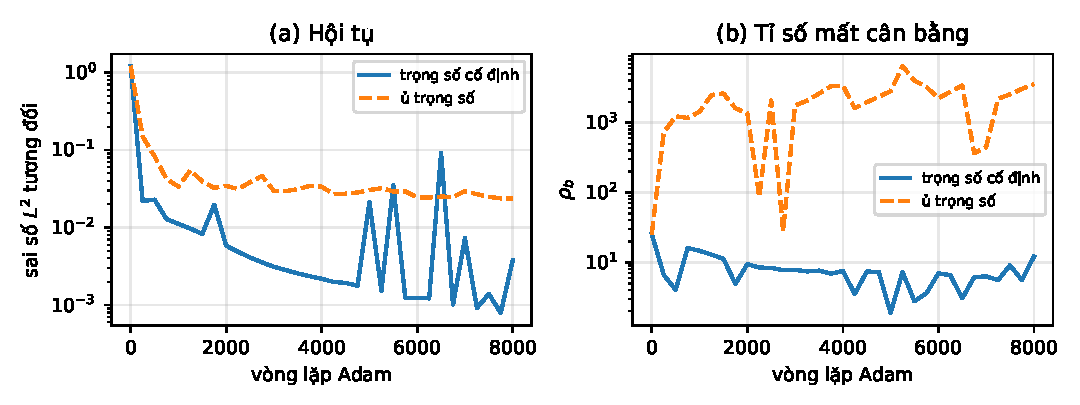
\includegraphics[width=\textwidth]{Images/chap_5/fig54_heat.pdf}
\caption{Phương trình khuếch tán. (a) Hội tụ sai số $L^2$ trong giai đoạn Adam.
(b) Chỉ số mất cân bằng $\rho_b$: với trọng số cố định, $\rho_b$ giảm dần -- theo
Định nghĩa~\ref{dn:rho}, đây là dấu hiệu không có bệnh lý gradient.}
\label{fig:tn4}
\end{figure}
 
\begin{nhanxet}[Điều kiện áp dụng của Thuật toán~\ref{alg:annealing}]
\label{nx:dieu-kien-anneal}
Kết quả trên không bác bỏ Thuật toán~\ref{alg:annealing} mà \emph{xác định phạm vi
áp dụng} của nó. Quy tắc \eqref{eq:lambda-hat} chỉ nhằm làm cân bằng biên độ
gradient; không có kết quả nào trong Chương~\ref{chap:pinn} khẳng định việc cân
bằng ấy luôn cải thiện độ chính xác, và Nhận xét~\ref{nx:danh-doi} đã cho một cơ
chế cụ thể khiến nó có thể làm xấu đi.
 
Khuyến nghị rút ra: \emph{đo $\rho_b$ trước, bật ủ trọng số sau}. Nếu $\rho_b$ nhỏ
hoặc có xu hướng giảm, giữ trọng số cố định. Chi phí của phép đo này, theo
Mục~\ref{ssec:rho}, là không đáng kể so với việc chạy hỏng cả một phiên huấn
luyện.
\end{nhanxet}
 
%==============================================================================
\section{Thí nghiệm 5: phương trình Burgers độ nhớt nhỏ}
\label{sec:tn5}
%==============================================================================
 
\begin{equation}
\left\{
\begin{aligned}
&\partial_t u + u\,\partial_x u - \nu\,\partial_{xx} u = 0,
  && (x,t) \in (-1,1)\times(0,1], \quad \nu = \tfrac{0{,}01}{\pi},\\
&u(x,0) = -\sin(\pi x), \quad u(-1,t) = u(1,t) = 0.
\end{aligned}
\right.
\label{eq:burgers-tn5}
\end{equation}
 
Đây là bài toán mà cả ba tầng của Bảng~\ref{tab:ba-nguyen-nhan} cùng bất lợi: hằng
số ổn định cỡ $1/(\pi^2\nu) \approx 31{,}8$, lớp trong đòi hỏi tần số
$\abs{k}\sim 77$, và toán tử bậc hai khuếch đại phổ theo $\norm{k}^2$.
 
\textbf{Nghiệm tham chiếu.} Bài toán \eqref{eq:burgers-tn5} không có nghiệm đóng
dạng sơ cấp, nên ta dựng nghiệm tham chiếu bằng sai phân hữu hạn bậc hai kết hợp
Runge--Kutta bậc bốn tường minh: dạng bảo toàn $\big(u^2/2\big)_x$ sai phân trung
tâm, khuếch tán sai phân trung tâm ba điểm, $N_x = 2\,047$ điểm trong,
$\Delta t = 5\times10^{-5}$. Số Péclet lưới
$\mathrm{Pe} = \max\abs{u}\,\Delta x/\nu \approx 0{,}31 < 2$ bảo đảm sai phân
trung tâm không dao động. Kiểm chứng hội tụ lưới bằng cách so với lần chạy
$N_x = 1\,023$ cho sai lệch $L^2$ tương đối $2{,}31\times10^{-4}$, nhỏ hơn hai bậc
so với sai số PINN cần đo, nên nghiệm tham chiếu đủ chính xác để làm chuẩn.
 
Nghiệm tham chiếu cho $\max_x\abs{\partial_x u} = 150{,}1$ tại $t = 0{,}5$, xác
nhận sự tồn tại của lớp trong sắc nét mà Mục~\ref{subsec:thang-do-dai} dự báo. Thời
điểm hình thành khớp với giá trị lý thuyết cho phương trình Burgers không nhớt,
$t_b = 1/\max\abs{u_0'} = 1/\pi \approx 0{,}318$.
 
\begin{nhanxet}[Cần thống nhất một nghiệm tham chiếu duy nhất]
\label{nx:hai-nghiem-tham-chieu}
Mục~\ref{subsec:thang-do-dai} trích $\max\abs{u_x} \approx 151$ tại
$t \approx 0{,}51$ từ một nghiệm giả phổ Fourier với $2\,048$ chế độ, còn mục này
trích $150{,}1$ tại $t = 0{,}5$ từ nghiệm sai phân hữu hạn. Hai con số nhất quán
với nhau trong phạm vi sai số của cả hai lược đồ, nhưng chúng đến từ \emph{hai
nghiệm tham chiếu khác nhau}. Khi hoàn thiện luận văn, cần chọn một nghiệm tham
chiếu duy nhất và dùng nó ở cả hai chương, đồng thời nêu rõ lược đồ và tham số rời
rạc hoá đúng một lần.
\end{nhanxet}
 
\textbf{Thiết lập PINN.} $N_r = 2\,500$, $N_b = 300$, $N_0 = 300$; $6\,000$ vòng
Adam rồi L-BFGS.
 
\begin{table}[H]
\centering
\caption{Phương trình Burgers \eqref{eq:burgers-tn5} so với nghiệm tham chiếu sai
phân hữu hạn.}
\label{tab:tn5}
\small
\begin{tabular}{@{}lrrrr@{}}
\toprule
\textbf{Chiến lược} & $\varepsilon_{L^2}$ (Adam) & $\varepsilon_{L^2}$ (cuối)
& $\varepsilon_{L^{\infty}}$ & $\lambda_b$ cuối \\
\midrule
Trọng số cố định
& $4{,}525\times10^{-2}$ & $\mathbf{2{,}837\times10^{-2}}$
& $4{,}348\times10^{-1}$ & $1{,}00$ \\
Ủ trọng số, $\alpha = 0{,}9$
& $6{,}230\times10^{-1}$ & $4{,}512\times10^{-1}$
& $1{,}008\times10^{0}$ & $6{,}01\times10^{4}$ \\
Ủ trọng số, $\alpha = 0{,}1$
& $5{,}959\times10^{-1}$ & $4{,}489\times10^{-1}$
& $1{,}037\times10^{0}$ & $1{,}45\times10^{5}$ \\
\bottomrule
\end{tabular}
\end{table}
 
\begin{figure}[H]
\centering
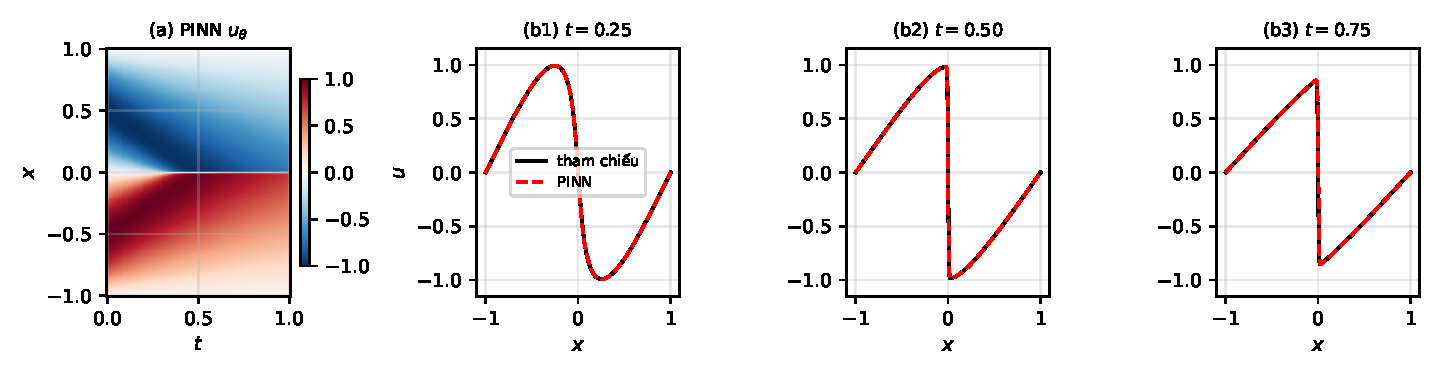
\includegraphics[width=\textwidth]{Images/chap_5/fig55_burgers.pdf}
\caption{Nghiệm PINN cho phương trình Burgers với $\nu = 0{,}01/\pi$. (a) Trường
nghiệm $u_{\btheta}(x,t)$. (b1)--(b3) Lát cắt theo thời gian so với nghiệm tham
chiếu.}
\label{fig:tn5}
\end{figure}
 
\textbf{Kết quả 1: bệnh lý gradient xuất hiện đúng như dự báo.}
Hình~\ref{fig:tn6}(a) cho phép so sánh trực tiếp hai bài toán:
\begin{equation}
\max\rho_b\big|_{\text{Burgers}} = 1\,758{,}2
\qquad\text{so với}\qquad
\max\rho_b\big|_{\text{khuếch tán}} = 25{,}4,
\label{eq:so-sanh-rho}
\end{equation}
tức chênh nhau $69{,}2$ lần. Quan trọng hơn con số tuyệt đối là \emph{xu hướng}:
với Burgers, $\rho_b$ \emph{tăng} từ $14{,}4$ tại khởi tạo lên $1\,758{,}2$ sau
$6\,000$ vòng, trong khi với khuếch tán nó giảm. Đây đúng là điều kiện thứ hai
trong Định nghĩa~\ref{dn:rho}, và nó chỉ xuất hiện ở bài toán cứng -- kết quả này
xác nhận bệnh lý gradient là hiện tượng \emph{phụ thuộc bài toán}, không phải đặc
tính cố hữu của mọi PINN.
 
\textbf{Kết quả 2: cơ chế khuếch đại -- quan sát chưa có chứng minh.} Ta đo
$\norm{\bW^{(1)}}_F$ tăng từ $1{,}83$ lên $3{,}68$, tức
$\norm{\bW^{(1)}}_F^2$ tăng $4{,}04$ lần, trong khi $\rho_b$ tăng $122$ lần. Hai
đại lượng cùng tăng đơn điệu và cùng lúc (Hình~\ref{fig:tn6}b), gợi ý một mối liên
hệ giữa chuẩn trọng số lớp vào và mức mất cân bằng gradient.
 
Cần nói rõ giới hạn của quan sát này. Luận văn \emph{không} có mệnh đề nào chứng
minh $\rho_b \sim \norm{\bW^{(1)}}^2$; đây là một tương quan quan sát được trên
một lần chạy, không phải một dự báo được kiểm chứng. Hệ số $4{,}04$ cũng không
giải thích được hệ số $122$, nên nếu có một quan hệ luỹ thừa thì số mũ phải lớn
hơn $1$ đáng kể. Một hướng giải thích khả dĩ, phù hợp với
Mệnh đề~\ref{md:jacobian}: $\partial_{xx}u_{\btheta}$ theo truy hồi
\eqref{eq:S-truy-hoi} chứa tích của các $\bW^{(\ell)}$ ở \emph{mọi} lớp, không chỉ
lớp đầu, nên chuẩn của một lớp không đủ để giải thích. Ta ghi nhận đây là câu hỏi
để ngỏ chứ không kết luận.
 
\begin{figure}[H]
\centering
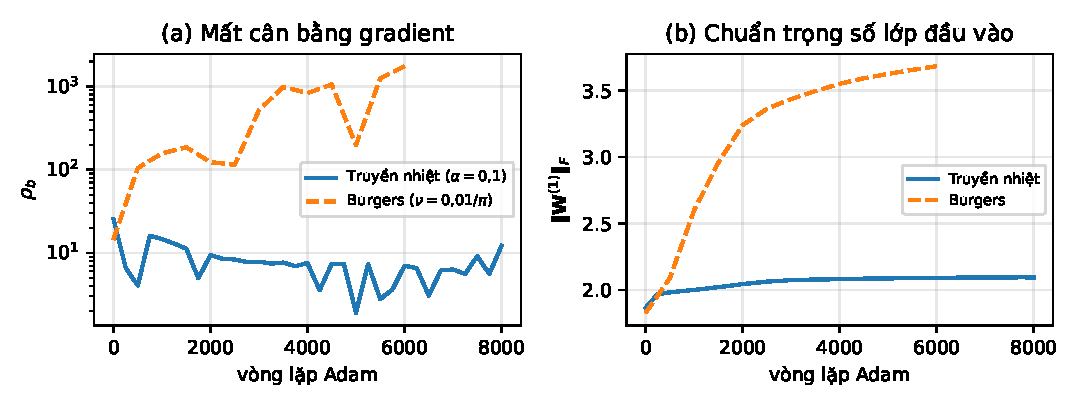
\includegraphics[width=\textwidth]{Images/chap_5/fig56_rho.pdf}
\caption{So sánh hai bài toán. (a) $\rho_b$ tăng đơn điệu với Burgers, giảm với
khuếch tán. (b) Chuẩn Frobenius của ma trận trọng số lớp vào.}
\label{fig:tn6}
\end{figure}
 
\textbf{Kết quả 3: ủ trọng số thất bại cả trên bài toán cứng.} Đây là kết quả cần
thận trọng nhất trong chương. Ủ trọng số làm sai số xấu đi $15{,}9$ lần
($2{,}84\times10^{-2} \to 4{,}51\times10^{-1}$), với $\lambda_b$ chạy tới
$6{,}01\times10^4$. Vì bài toán này \emph{thực sự} có bệnh lý gradient theo
\eqref{eq:so-sanh-rho}, không thể giải thích bằng
Nhận xét~\ref{nx:dieu-kien-anneal}.
 
Trước khi kết luận, ta loại trừ hai giả thuyết cạnh tranh.
 
\emph{(i) Sai công thức?} Công thức cài đặt trùng với \eqref{eq:lambda-hat} của
Chương~\ref{chap:pinn}, vốn được đối chiếu trực tiếp với Thuật toán 2.1
của~\cite{wang2021}.
 
\emph{(ii) Sai hệ số làm trơn?} Với quy tắc \eqref{eq:lambda-update}, giá trị
$\alpha$ nhỏ làm trơn mạnh còn $\alpha$ gần $1$ nghiêng hẳn về ước lượng mới; bài
báo gốc khuyến nghị $\alpha = 0{,}1$. (Ký hiệu $\alpha$ ở đây là hệ số làm trơn
của \eqref{eq:lambda-update}, không liên quan tới hệ số khuếch tán $\nu$ của
\eqref{eq:heat}.) Ta chạy lại với cả hai giá trị. Hai dòng cuối
Bảng~\ref{tab:tn5} cho kết quả gần như nhau ($4{,}51\times10^{-1}$ so với
$4{,}49\times10^{-1}$), nên kết luận không nhạy với lựa chọn này.
 
Nguyên nhân thực sự là một \emph{bất ổn định phản hồi dương} nằm ngay trong cấu
trúc của quy tắc \eqref{eq:lambda-hat}, và có thể chứng minh được.
 
\begin{bode}[Phản hồi dương của quy tắc cân bằng trọng số]
\label{bd:phan-hoi-duong}
Giả sử thành phần thứ $i$ có dạng
$J_i(\btheta) = \frac{1}{N_i}\sum_{j=1}^{N_i} g_j(\btheta)^2$ với
$g_j \in C^1$ và $\norm{\nabla g_j(\btheta)} \le G_i$ trên miền đang xét. Khi đó
\begin{equation}
\norm{\nabla_{\btheta} J_i(\btheta)}_{1}
 \;\le\; 2\,G_i\,\sqrt{P}\;\sqrt{J_i(\btheta)} ,
\label{eq:grad-le-sqrt}
\end{equation}
và do đó, với $\hat\lambda_i$ cho bởi \eqref{eq:lambda-hat},
\begin{equation}
\hat{\lambda}_i(\btheta)
 \;\ge\; \frac{\sqrt{P}\;\norm{\nabla_{\btheta}J_r(\btheta)}_{\infty}}
              {2G_i}\cdot\frac{1}{\sqrt{J_i(\btheta)}}
 \;\xrightarrow[\;J_i \to 0\;]{}\; +\infty ,
\label{eq:lambda-phan-ky}
\end{equation}
miễn là $\norm{\nabla_{\btheta}J_r}_{\infty}$ bị chặn dưới bởi một hằng số dương.
\end{bode}
 
\begin{proof}
Ta có $\nabla J_i = \frac{2}{N_i}\sum_j g_j \nabla g_j$, nên theo bất đẳng thức
tam giác rồi Cauchy--Schwarz trên chỉ số $j$,
\begin{align*}
\norm{\nabla J_i}_{2}
 &\le \frac{2}{N_i}\sum_j \abs{g_j}\,\norm{\nabla g_j}_2
  \le \frac{2G_i}{N_i}\sum_j \abs{g_j}
  \le \frac{2G_i}{N_i}\sqrt{N_i}\Big(\sum_j g_j^2\Big)^{1/2}\\
 &= \frac{2G_i}{N_i}\sqrt{N_i}\cdot\sqrt{N_i J_i}
  = 2G_i\sqrt{J_i},
\end{align*}
trong đó bước cuối dùng $\sum_j g_j^2 = N_i J_i$ theo định nghĩa của $J_i$.
Chuyển sang chuẩn $L^1$ trên $\R^P$ bằng
$\norm{\bm{v}}_1 \le \sqrt{P}\,\norm{\bm{v}}_2$ cho
\eqref{eq:grad-le-sqrt}. Thay vào mẫu số của \eqref{eq:lambda-hat}, vốn bằng
$\tfrac{1}{P}\norm{\nabla J_i}_1$, được \eqref{eq:lambda-phan-ky}.
\end{proof}
 
Bổ đề~\ref{bd:phan-hoi-duong} cho chính xác cơ chế hỏng. Khi $J_i$ giảm, mẫu số
của \eqref{eq:lambda-hat} giảm ít nhất theo $\sqrt{J_i}$, làm $\hat{\lambda}_i$
tăng, khiến thành phần $i$ được ưu tiên hơn nữa và $J_i$ giảm nhanh hơn nữa. Vòng
phản hồi này \emph{không có cơ chế tự hãm}: cận dưới \eqref{eq:lambda-phan-ky}
phân kỳ như $J_i^{-1/2}$.
 
Số liệu khớp với dự báo. Trong lần chạy có ủ, $\rho_b$ đạt $1{,}69\times10^5$, tức
cao gấp $96$ lần lần chạy không ủ -- thuật toán nhằm \emph{giảm} mất cân bằng lại
làm nó trầm trọng hơn hai bậc độ lớn. Và theo
Nhận xét~\ref{nx:danh-doi}, $\lambda_b$ ở thang $10^4$--$10^5$ nằm xa quá mức giá
trị hữu hạn tối ưu, nên phần dư trong miền bị hy sinh hoàn toàn.
 
\begin{nhanxet}[Kết luận thực hành về ủ trọng số]
\label{nx:ket-luan-anneal}
Trên cả hai bài toán khảo sát, Thuật toán~\ref{alg:annealing} ở dạng nguyên bản
đều làm giảm độ chính xác, và Bổ đề~\ref{bd:phan-hoi-duong} cho thấy đây không
phải trùng hợp mà là hệ quả cấu trúc của quy tắc \eqref{eq:lambda-hat} khi
$J_i \to 0$. Hai hướng khắc phục theo đúng cơ chế vừa chứng minh: đặt chặn trên
cho $\lambda_i$, hoặc thay mẫu số bằng một đại lượng không triệt tiêu cùng $J_i$
-- chẳng hạn vết của nhân tiếp tuyến thay cho chuẩn gradient.
 
Với phạm vi luận văn này, khuyến nghị là dùng trọng số cố định kèm dò tìm
$\lambda_b$ theo Bảng~\ref{tab:tn2}, và xem việc ủ trọng số như một hướng cần khảo
sát thêm. Cần nêu rõ rằng kết luận này \emph{không} bác bỏ kết quả
của~\cite{wang2021}, vốn báo cáo cải thiện hơn một bậc độ lớn trên bài toán
Helmholtz: sự khác biệt có thể nằm ở bài toán, ở ngân sách huấn luyện, hoặc ở chi
tiết cài đặt mà ta chưa tái lập được. Điều Bổ đề~\ref{bd:phan-hoi-duong} khẳng
định là quy tắc có một chế độ hỏng xác định, không phải là nó luôn hỏng.
\end{nhanxet}
 
\textbf{Kết quả 4: chất lượng nghiệm.} Với trọng số cố định, PINN đạt
$\varepsilon_{L^2} = 2{,}84\times10^{-2}$.
Hình~\ref{fig:tn5}(b2)--(b3) cho thấy lớp trong tại $x = 0$ được tái tạo. Chênh
lệch lớn giữa $\varepsilon_{L^2} = 2{,}84\times10^{-2}$ và
$\varepsilon_{L^{\infty}} = 4{,}35\times10^{-1}$ -- hệ số $15$ lần -- có ý nghĩa
cấu trúc: sai số hầu như tập trung toàn bộ vào một dải hẹp quanh $x = 0$, đúng như
phân tích ba tầng ở Bảng~\ref{tab:ba-nguyen-nhan} dự báo. Bậc sai số trung bình
vẫn chấp nhận được, nhưng đúng chỗ quan trọng nhất về mặt vật lý thì sai số lớn
nhất.
 
%==============================================================================
\section{Thí nghiệm 6: kiểm chứng chặn ổn định}
\label{sec:tn6}
%==============================================================================

\begin{thinghiem}[Kiểm chứng Mệnh đề~\ref{md:chan-on-dinh}]
\label{tn:chan}
Mệnh đề~\ref{md:chan-on-dinh} là mắt xích biện minh cho toàn bộ phương pháp: nó
nói rằng cực tiểu hoá một đại lượng \emph{tính được} ($\norm{r_{\btheta}}$) khống
chế được đại lượng \emph{quan tâm} ($\norm{e_{\btheta}}$). Nhưng chặn ấy có một
giả thiết dễ bị bỏ qua: điều kiện biên phải được thoả \emph{chính xác}. Câu hỏi:
chặn có đúng trong thực tế không, nó chặt đến đâu, và điều gì xảy ra khi giả
thiết bị vi phạm?
\end{thinghiem}

\textbf{Thiết lập.} Vẫn bài toán Poisson \eqref{eq:poisson-tn1}. Ta đo đồng thời
$\norm{r_{\btheta}}_{L^2}$, $\norm{e_{\btheta}}_{L^2}$ và
$\norm{e_{\btheta}'}_{L^2}$ trên lưới đánh giá $20\,001$ điểm bằng quy tắc hình
thang, tại sáu mốc trải suốt quá trình huấn luyện để quét được bốn bậc độ lớn
của phần dư. Ba cấu hình tách bạch vai trò của giả thiết:

\begin{enumerate}[label=(\alph*),leftmargin=2.2em,itemsep=2pt]
\item \textbf{Ràng buộc cứng} $\hat u_{\btheta}(x) = x(1-x)\,u_{\btheta}(x)$ theo
Bổ đề~\ref{bd:rang-buoc-cung}, với $D(x) = x(1-x)$ đúng như dạng được đề nghị ở
Mục~\ref{subsec:rang-buoc}. Điều kiện biên thoả chính xác với mọi $\btheta$, tức
giả thiết của mệnh đề được \emph{thoả theo cấu trúc}.
\item \textbf{Ràng buộc mềm, $\lambda_b = 100$} -- giá trị tốt nhất theo
Bảng~\ref{tab:tn2}. Giả thiết chỉ thoả gần đúng.
\item \textbf{Ràng buộc mềm, $\lambda_b = 0{,}01$} -- giá trị mà
Bảng~\ref{tab:tn2} cho thấy sai số biên bão hoà ở mức $0{,}91$. Giả thiết bị vi
phạm nặng.
\end{enumerate}

\begin{table}[H]
\centering
\caption[Kiểm chứng chặn ổn định của Mệnh đề~\ref{md:chan-on-dinh}]{Kiểm chứng
chặn $\norm{e_{\btheta}}_{L^2} \le \pi^{-2}\norm{r_{\btheta}}_{L^2}$. Cột
``tỉ số'' là $\norm{e_{\btheta}}_{L^2}/\norm{r_{\btheta}}_{L^2}$; chặn được thoả
khi tỉ số này không vượt $\pi^{-2} \approx 0{,}1013$.}
\label{tab:tn6}
\small
\setlength{\tabcolsep}{4pt}
\begin{tabular}{@{}l rrr r c@{}}
\toprule
\textbf{Mốc} & $\norm{r_{\btheta}}_{L^2}$ & $\norm{e_{\btheta}}_{L^2}$
& sai số biên & tỉ số & thoả chặn? \\
\midrule
\multicolumn{6}{@{}l}{\emph{(a) Ràng buộc cứng --- giả thiết thoả chính xác}}\\
Khởi tạo   & $2{,}809\times10^{1}$ & $7{,}115\times10^{-1}$ & $0$ & $0{,}0253$ & có \\
Adam $200$ & $5{,}735\times10^{0}$ & $3{,}705\times10^{-2}$ & $0$ & $0{,}0065$ & có \\
Adam $1000$& $1{,}511\times10^{-1}$& $4{,}173\times10^{-4}$ & $0$ & $0{,}0028$ & có \\
Adam $4000$& $2{,}526\times10^{-2}$& $6{,}109\times10^{-5}$ & $0$ & $0{,}0024$ & có \\
$+$ L-BFGS & $2{,}599\times10^{-3}$& $1{,}815\times10^{-6}$ & $0$ & $0{,}0007$ & có \\
\addlinespace
\multicolumn{6}{@{}l}{\emph{(b) Ràng buộc mềm, $\lambda_b = 100$}}\\
Adam $1000$& $1{,}663\times10^{-1}$& $7{,}820\times10^{-3}$ & $1{,}7\times10^{-2}$ & $0{,}0470$ & có \\
$+$ L-BFGS & $4{,}214\times10^{-3}$& $5{,}029\times10^{-6}$ & $9{,}9\times10^{-6}$ & $0{,}0012$ & có \\
\addlinespace
\multicolumn{6}{@{}l}{\emph{(c) Ràng buộc mềm, $\lambda_b = 0{,}01$}}\\
Adam $200$ & $4{,}033\times10^{0}$ & $2{,}923\times10^{0}$  & $5{,}21$ & $0{,}7248$ & \textbf{không} \\
Adam $1000$& $9{,}087\times10^{-2}$& $8{,}736\times10^{-1}$ & $1{,}52$ & $\mathbf{9{,}614}$ & \textbf{không} \\
Adam $4000$& $2{,}976\times10^{-2}$& $2{,}906\times10^{-1}$ & $0{,}503$& $\mathbf{9{,}763}$ & \textbf{không} \\
$+$ L-BFGS & $4{,}304\times10^{-3}$& $1{,}127\times10^{-3}$ & $2{,}1\times10^{-3}$ & $0{,}2618$ & \textbf{không} \\
\bottomrule
\end{tabular}
\end{table}

\textbf{Kết quả.} Ba kết luận, mỗi kết luận trả lời một phần của câu hỏi đặt ra.

\emph{(a) Chặn đúng, và đúng trên toàn dải.} Với ràng buộc cứng, tỉ số
$\norm{e_{\btheta}}/\norm{r_{\btheta}}$ nằm dưới $\pi^{-2}$ tại \emph{mọi} mốc,
trong khi $\norm{r_{\btheta}}$ quét bốn bậc độ lớn từ $2{,}81\times10^{1}$ xuống
$2{,}60\times10^{-3}$. Chặn cho đạo hàm cũng đúng: tỉ số
$\norm{e_{\btheta}'}/\norm{r_{\btheta}}$ cao nhất là $0{,}159$, dưới
$\pi^{-1}\approx 0{,}318$.

\emph{(b) Chặn không chặt.} Tỉ số quan sát được nằm trong khoảng
$0{,}0007$--$0{,}0261$, tức nhỏ hơn hằng số $\pi^{-2}$ từ $4$ đến $145$ lần. Điều
này không mâu thuẫn với mệnh đề: hằng số $\pi^{-2}$ là tối ưu trên \emph{toàn bộ}
lớp hàm $H^1_0(0,1)$, đạt được khi sai số trùng hàm riêng $\sin \pi x$ ứng với
trị riêng nhỏ nhất. Sai số của mạng nơ-ron ở đây không có dạng ấy, nên chặn còn
dư địa. Hệ quả thực hành: chặn dùng được như một \emph{bảo đảm}, không dùng được
như một \emph{ước lượng} sai số.

\emph{(c) Giả thiết điều kiện biên là thiết yếu, không phải trang trí.} Với
$\lambda_b = 0{,}01$, chặn bị vi phạm ở mọi mốc sau khởi tạo, và mức vi phạm lên
tới $9{,}76$ so với $0{,}1013$ --- tức \emph{gấp $96$ lần}. Đọc dòng
``Adam $4000$'' cho thấy rõ cơ chế: phần dư đã nhỏ
($\norm{r_{\btheta}} = 2{,}98\times10^{-2}$) trong khi sai số vẫn lớn
($\norm{e_{\btheta}} = 2{,}91\times10^{-1}$, gấp mười lần phần dư). Đây chính là
kịch bản mà Nhận xét~\ref{rem:ill-posedness} mô tả: mạng trôi trên tập
$\mathcal{M}_r$ của \eqref{eq:manifold-r} và hội tụ về \emph{một nghiệm khác} của
cùng phương trình vi phân.

\begin{nhanxet}[Vì sao thí nghiệm này đáng làm]
\label{nx:y-nghia-tn6}
Đây là thí nghiệm duy nhất trong chương kiểm chứng trực tiếp mắt xích
\emph{logic} của phương pháp chứ không phải một hiện tượng của mô hình. Nó cho
một quy tắc thực hành cụ thể: chỉ khi điều kiện biên được thoả (chính xác bằng
ràng buộc cứng, hoặc tới độ chính xác cao bằng $\lambda_b$ đủ lớn) thì việc theo
dõi $J_r$ mới là chỉ báo hợp lệ cho sai số. Ở chế độ $\lambda_b$ nhỏ, một giá trị
$J_r$ nhỏ \emph{không} nói gì về chất lượng nghiệm --- và đó là chế độ mà bệnh lý
gradient (Mục~\ref{sec:gradient-pathology}) tự động đẩy bài toán vào khi
$\lambda_b$ không được chọn cẩn thận.
\end{nhanxet}

%==============================================================================
\section{Đối chiếu lý thuyết và thực nghiệm}
\label{sec:doi-chieu}
%==============================================================================
 
\begin{table}[H]
\centering
\caption{Đối chiếu giữa các kết quả lý thuyết và số liệu đo được.}
\label{tab:doi-chieu}
\small
\begin{tabular}{@{}p{2.9cm}p{3.7cm}p{3.9cm}p{3.0cm}@{}}
\toprule
\textbf{Kết quả} & \textbf{Dự báo} & \textbf{Đo được} & \textbf{Kết luận} \\
\midrule
Hệ quả~\ref{hq:pinn-hong}
& $\nabla_{\btheta}J_r \equiv \bm{0}$ với ReLU
& $\norm{\nabla J_r}_\infty = 0{,}0$; $J_r = 776{,}23$ so với $778{,}49$ trên
  lưới đánh giá
& \textbf{Khớp chính xác} \\[4pt]
Mệnh đề~\ref{md:phat-bien-phat}
& sai số biên $\propto \lambda_b^{-1}$
& số mũ đo được $-0{,}907$; bão hoà ở hai đầu
& \textbf{Khớp}, lệch $9\%$ ở số mũ \\[4pt]
Mục~\ref{subsec:adam-vs-lbfgs}
& tựa Newton vượt điều kiện số xấu và sàn nhiễu
& cải thiện $28{,}6$ lần sau $500$ vòng
& \textbf{Khớp} \\[4pt]
Định nghĩa~\ref{dn:rho}
& bệnh lý chỉ ở bài toán cứng
& $\rho_b$: $1\,758$ (Burgers) so với $25{,}4$ (khuếch tán); xu hướng ngược nhau
& \textbf{Khớp} \\[4pt]
Giả thuyết \eqref{eq:pho-hieu-dung}
& phần dư ưu tiên $k$ cao
& $\abs{c_1}/\abs{c_8} = 38{,}6$; thứ tự học đảo chiều so với hồi quy
& \textbf{Khớp về hướng} \\[4pt]
Mục~\ref{subsec:he-qua-pinn}
& lớp sốc học chậm nhất
& với Poisson thì ngược lại
& \textbf{Cần siết lại} (Nhận xét~\ref{nx:hieu-chinh}) \\[4pt]
Quan hệ $\rho_b$--$\norm{\bW^{(1)}}^2$
& (không có mệnh đề)
& $\norm{\bW^{(1)}}^2$ tăng $4{,}04$ lần, $\rho_b$ tăng $122$ lần
& \textbf{Tương quan}, chưa giải thích \\[4pt]
Thuật toán~\ref{alg:annealing}
& cân bằng biên độ gradient
& làm xấu $35{,}6$ lần (khuếch tán), $15{,}9$ lần (Burgers)
& \textbf{Có chế độ hỏng} (Bổ đề~\ref{bd:phan-hoi-duong}) \\[4pt]
Mệnh đề~\ref{md:chan-on-dinh}
& $\norm{e}_{L^2}\le \pi^{-2}\norm{r}_{L^2}$ khi điều kiện biên thoả chính xác
& tỉ số $\le 0{,}026$ trên bốn bậc độ lớn của $\norm{r}$; vi phạm $96$ lần khi
  $\lambda_b = 0{,}01$
& \textbf{Khớp}, và giả thiết biên tỏ ra thiết yếu \\
\bottomrule
\end{tabular}
\end{table}
 
Trong chín hạng mục: năm khớp trọn vẹn, một khớp về hướng nhưng không rút được
kết luận định lượng, một cần siết lại cách phát biểu, một chỉ là tương quan chưa
giải thích được, và một cho kết quả tiêu cực nhưng đã truy được nguyên nhân.
 
Mức khớp này ủng hộ khung lý thuyết của Chương~\ref{chap:pinn} một cách
\emph{có điều kiện}, và điều kiện ấy đáng được nêu rõ: bốn trong năm hạng mục
khớp trọn vẹn tương ứng với một mệnh đề \emph{đã được chứng minh}
(Hệ quả~\ref{hq:pinn-hong}, Mệnh đề~\ref{md:phat-bien-phat},
Mệnh đề~\ref{md:san-nhieu}, Mệnh đề~\ref{md:chan-on-dinh}); hạng mục còn lại dựa trên
Định nghĩa~\ref{dn:rho}, vốn là một \emph{tiêu chí chẩn đoán} do luận văn đặt ra
chứ không phải một mệnh đề, nên nó kiểm chứng tính hữu dụng của tiêu chí chứ
không kiểm chứng một dự báo lý thuyết. Ngược lại, cả ba hạng mục có vấn đề đều
tương ứng với những chỗ luận văn dùng \emph{suy luận tiệm cận} hoặc \emph{ghép
hai kết quả rời rạc}:
giả thuyết \eqref{eq:pho-hieu-dung} ghép $\abs{P}^2$ với
$\widehat{\varkappa}$; kết luận ở Mục~\ref{subsec:he-qua-pinn} ngầm giả định thừa
số nào thắng; quan hệ $\rho_b$--$\norm{\bW^{(1)}}^2$ không có chứng minh nào cả.
 
Đây là bài học phương pháp luận của chương, và nó nhất quán với ranh giới mà
Chương~\ref{chap:fnn} đã vạch giữa lý thuyết xấp xỉ và lý thuyết tối ưu: những gì
được chứng minh thì đứng vững, những gì được suy đoán thì cần kiểm chứng trước khi
dùng.
 
%==============================================================================
\section{Hạn chế của thiết kế thực nghiệm}
\label{sec:hanche}
%==============================================================================
 
Để các kết luận trên được đọc đúng phạm vi, cần nêu rõ những hạn chế sau.
 
\begin{enumerate}[label=(\arabic*),leftmargin=2.2em,itemsep=4pt]
\item \emph{Một hạt giống ngẫu nhiên duy nhất.} Mọi lần chạy dùng một hạt giống cố
định để tái lập được, nên không có ước lượng độ phân tán giữa các lần khởi tạo.
Đây là vi phạm trực tiếp nguyên tắc đã nêu ở Nhận xét~\ref{nx:doi-xung-hoan-vi}:
với ít nhất $2^{n_1}n_1!$ cực tiểu tương đương, một kết quả tốt từ một hạt giống
may mắn không phải bằng chứng về phương pháp. Hệ quả thực hành cho việc đọc chương
này: các chênh lệch dưới hai lần trong bảng số liệu \emph{không nên} được coi là
có ý nghĩa; mọi kết luận ở Mục~\ref{sec:doi-chieu} đều dựa trên chênh lệch từ một
bậc độ lớn trở lên. Khắc phục đúng cách là lặp mỗi cấu hình trên $5$--$10$ hạt
giống và báo cáo trung vị cùng khoảng phân vị.
 
\item \emph{Ngân sách huấn luyện hạn chế.} Toàn bộ thí nghiệm chạy trên một lõi
CPU, với $4\,000$--$8\,000$ vòng Adam, so với bậc $10^5$ vòng thường dùng trong
các công trình gốc~\cite{raissi2019}. Sai số Burgers $2{,}84\times10^{-2}$ vì vậy
\emph{không} phản ánh giới hạn của phương pháp PINN mà phản ánh giới hạn của ngân
sách; các công trình gốc báo cáo bậc $10^{-3}$--$10^{-4}$ trên cùng bài toán với
mạng lớn hơn và huấn luyện lâu hơn.
 
\item \emph{Mạng nhỏ.} Kiến trúc $2\,209$--$8\,513$ tham số nhỏ hơn đáng kể so với
chuẩn mực trong tài liệu. Nói riêng, lập luận NTK ở Nhận xét~\ref{rem:ntk-view}
giả thiết chế độ nhân tiếp tuyến \emph{hằng} (mạng vô hạn rộng); với mạng cỡ này
giả thiết ấy chỉ đúng gần đúng, nên Thí nghiệm~\ref{tn:pho} phải được hiểu là kiểm
chứng \emph{định tính} về thứ tự học, không phải kiểm chứng định lượng phổ NTK.
Đây cũng là lý do ta không rút kết luận số từ đối chiếu $38{,}6$ với $64$ ở
Mục~\ref{sec:tn3}.
 
\item \emph{Chưa khảo sát độ nhạy theo cách lấy mẫu.} Cả lấy mẫu siêu khối Latin
lẫn lấy mẫu thích nghi RAR ở Bảng~\ref{tab:remedies} đều chưa được kiểm chứng.
Riêng với bài toán Burgers ở Mục~\ref{sec:tn5}, nơi sai số tập trung vào một
dải hẹp quanh
$x = 0$, RAR là kỹ thuật có khả năng cải thiện rõ nhất và đáng được thử trước
tiên.
 
\item \emph{Nghiệm tham chiếu cho Burgers là nghiệm số.} Dù đã kiểm chứng hội tụ
lưới ($2{,}31\times10^{-4}$), đây vẫn không phải nghiệm giải tích, nên kết luận về
Burgers có thêm một tầng sai số so với bài toán khuếch tán ở
Mục~\ref{sec:tn4}. Thêm vào đó,
Nhận xét~\ref{nx:hai-nghiem-tham-chieu} đã nêu việc hai chương hiện dùng hai nghiệm
tham chiếu khác nhau.
 
\item \emph{Chặn ổn định mới được kiểm chứng ở trường hợp đơn giản nhất.}
Mục~\ref{sec:tn6} đã kiểm chứng Mệnh đề~\ref{md:chan-on-dinh} trên bài toán
Poisson. Nhưng Mệnh đề~\ref{md:chan-suy-bien} --- vốn mới là tầng thứ nhất của
Bảng~\ref{tab:ba-nguyen-nhan} --- thì chưa: sự suy biến của hằng số ổn định theo
$1/\nu$ đòi hỏi quét $\nu$ trên bài toán đối lưu--khuếch tán, và phép quét ấy
chưa được thực hiện. Đây là bổ sung có giá trị nhất còn lại cho chương này.
\end{enumerate}
 
%==============================================================================
\section*{Kết luận chương}
\addcontentsline{toc}{section}{Kết luận chương}
%==============================================================================
 
Chương này đã hiện thực hoá khung lý thuyết của Chương~\ref{chap:pinn} trên
PyTorch và đưa ra số liệu kiểm chứng cho từng phát biểu chính.
 
Về mặt \emph{kỹ thuật}, cơ chế đồ thị động cùng cờ \texttt{create\_graph=True} đủ
để hiện thực trực tiếp các truy hồi \eqref{eq:G-truy-hoi} và
\eqref{eq:S-truy-hoi} mà không cần lập trình tường minh $\sigma''$, đúng như
Mệnh đề~\ref{md:ad-tai-tao} bảo đảm; độ chính xác kép là điều kiện cần để phân
biệt sai số xấp xỉ với sai số làm tròn.
 
Về mặt \emph{kiểm chứng}, ba kết quả nổi bật. Thứ nhất,
Hệ quả~\ref{hq:pinn-hong} được xác nhận tới từng chữ số máy: mạng ReLU cho
gradient bằng đúng không, chứng tỏ điều kiện $\sigma \in C^m$ là bắt buộc chứ
không phải khuyến nghị. Thứ hai, bệnh lý gradient được chứng minh là hiện tượng
\emph{phụ thuộc bài toán}: $\rho_b$ chênh nhau $69$ lần giữa Burgers và khuếch
tán, và quan trọng hơn là ngược chiều xu hướng -- nên việc chẩn đoán trước khi can
thiệp là bắt buộc. Thứ ba, giả thuyết \eqref{eq:pho-hieu-dung} được xác nhận theo
cách bất ngờ nhất: toán tử vi phân \emph{đảo ngược} thiên kiến phổ, khiến sai số
dồn về mode tần số thấp; phát hiện này buộc phải siết lại cách phát biểu ở
Mục~\ref{subsec:he-qua-pinn}.
 
Về mặt \emph{phương pháp}, hai kết quả tiêu cực có giá trị riêng. Việc tăng
$\lambda_b$ vô hạn không phải chiến lược tốt, vì sai số $L^2$ toàn cục đạt cực
tiểu tại một giá trị hữu hạn -- điều mà Mệnh đề~\ref{md:phat-bien-phat}, vốn chỉ
theo dõi sai số biên, không thể tiên đoán. Và thuật toán ủ trọng số ở dạng nguyên
bản làm giảm độ chính xác trên cả hai bài toán; ở đây thực nghiệm không chỉ phát
hiện vấn đề mà còn dẫn tới một kết quả lý thuyết mới:
Bổ đề~\ref{bd:phan-hoi-duong} chứng minh rằng quy tắc \eqref{eq:lambda-hat} có một
chế độ phản hồi dương với tốc độ phân kỳ $\hat\lambda_i \sim J_i^{-1/2}$ và không
có cơ chế tự hãm.
 
Kết quả cuối cùng ấy minh hoạ đúng vai trò của chương: bước kiểm chứng số không
chỉ xác nhận hay bác bỏ lý thuyết đã có, mà còn chỉ ra chỗ lý thuyết cần được bổ
sung.
 
